\section{Installation}
To use it you need the following to be installed on your system
\begin{itemize}
    \item \codet{Python 2.7.x} or \codet{Python >=3.5}
    \item Packages for \codet{Python}:
            \begin{itemize}
                \item \codet{Tkinter}
            \end{itemize}
\end{itemize} 
Most probably all of the above packages are already installed provided \codet{Python}
is installed on your system.

Provided you've unpacked this package into \codet{<package\tus dir}, change to the
\codet{<package\tus dir/src} directory. There you will find the file named \codet{caenccf}.
You may need to make it executable. In linux the following command does the work:
\begin{lstlisting}
> chmod +x caenccf
\end{lstlisting}
Now just run it
\begin{lstlisting}
> ./caenccf
\end{lstlisting}
If everything is OK you should see the following window on your screen:
\begin{figure}[H]
    \centering
    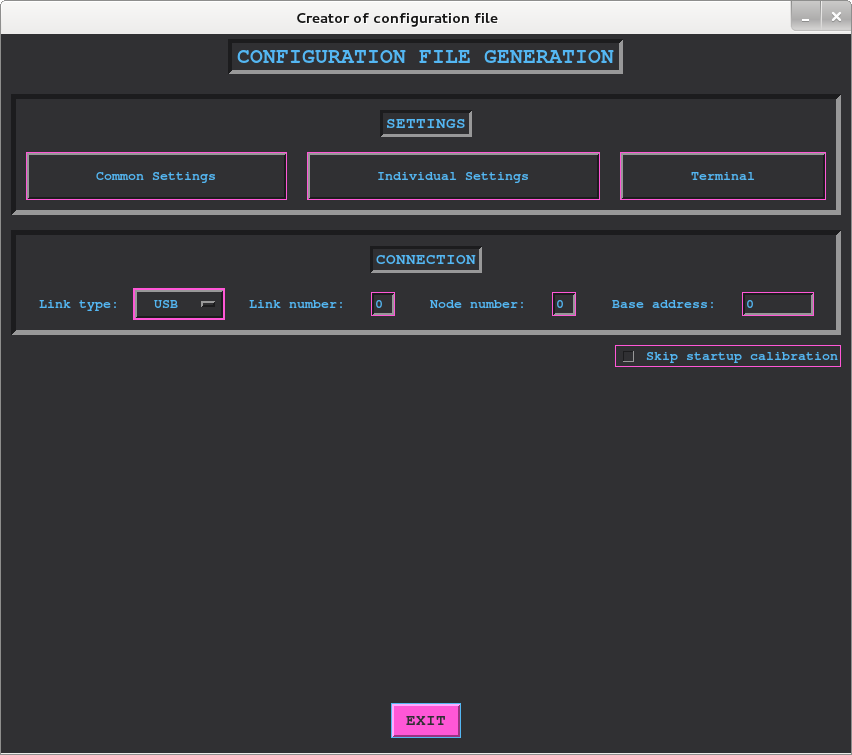
\includegraphics[width=0.8\textwidth]{../pictures/documentation/gui/start_page.png}
    \caption{GUI starting page}
    \label{fig:gui_stpg}
\end{figure}

It is very useful to be able to run it from everywhere on your system. In order to reach
this you need to place the executable in your \codet{bin} directory:
\begin{lstlisting}
> cp caenccf /usr/bin/
\end{lstlisting}
Also you need to extend the \codet{PYTHONPATH} environment variable in order \codet{Python}
to see necessary modules. Add the following lines in your \codet{.profile} (or \codet{.bash\tus profile}) file:
\begin{lstlisting}
if [[ -n "$PYTHONPATH" ]]; then
    PYTHONPATH=$PYTHONPATH:/path/to/<package_dir>/src
else
    export PYTHONPATH=/home/path/to/<package_dir>/src
fi;
\end{lstlisting}
Log out and log in back. After that you should be able to run the GUI from anywhere on your system. 
